%! Author = adnansiddiquei
%! Date = 19/03/2024

\section{Q1 - TESS Lightcurve}\label{sec:q1}
Using photometry data to identify exoplanets works through analysing the light curve of a star and identifying
periodic dips in the light intensity.
These dips are caused by the planet passing in front of the star, blocking some of the light, resulting in a
reduction in measured flux.
There are a variety of methods to find and fit for exoplanets, in this report, the \texttt{TLS} algorithm~\cite{hippke2019}
is used to analyse the provided TESS light curve data.

\begin{figure}[htb]
    \centering
    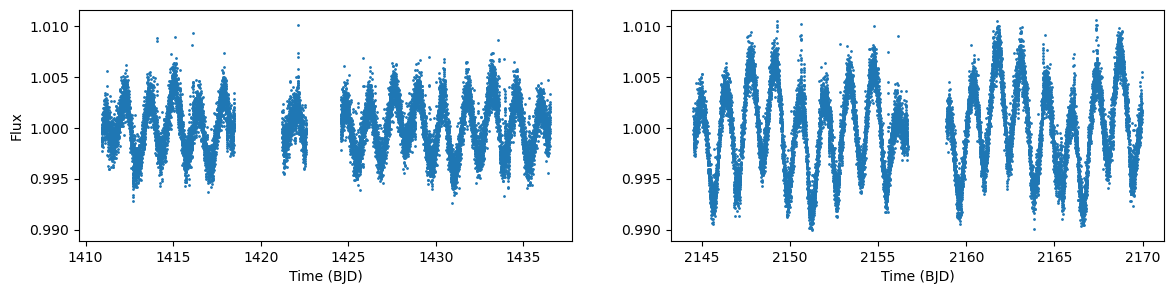
\includegraphics[width=1\textwidth]{figures/original_lightcurve}
    \caption{The original TESS light curve data, after outliers have been removed. The data is split into two
    plots as there is a large time gap between the two sets of data.}
    \label{fig:original_lightcurve}
\end{figure}

First, the data is pre-processed by removing any outliers, which were classified as points that are more than 3 standard
deviations away from the median.
This data is shown in Figure~\eqref{fig:original_lightcurve}, where it is apparent that a short term periodicity is
present in the data.
This periodicity is due to stellar activity, most likely due to the rotation of the star and as such it needs to be normalised
out before any exoplanets can be identified.
The TLS algorithm is then used to identify the strongest period, which is the aforementioned stellar activity.

\begin{figure}
\centering
\begin{subfigure}{0.5\textwidth}
    \centering
    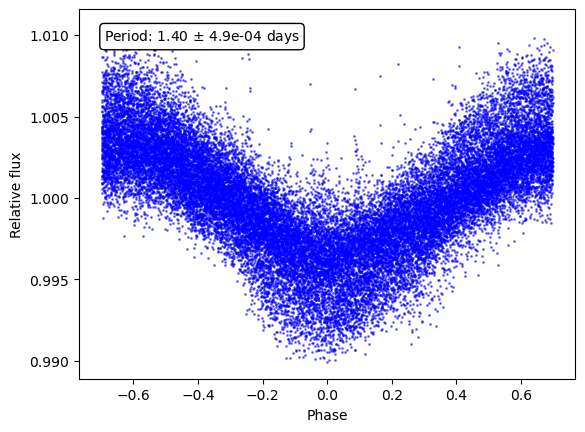
\includegraphics[width=1\textwidth]{figures/tls_results_0}
    \caption{The folded lightcurve of the strongest period identified by the TLS algorithm. The period is 1.40 days.}
    \label{fig:tls_results_0_folded}
\end{subfigure}%
\hfill
\begin{subfigure}{0.75\textwidth}
    \centering
    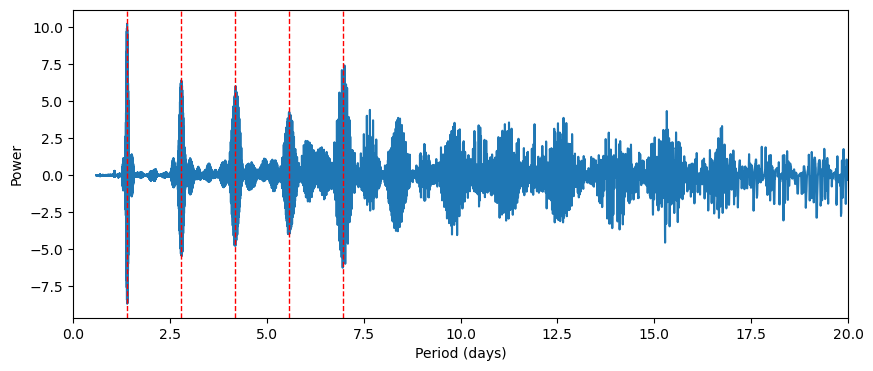
\includegraphics[width=1\textwidth]{./figures/tls_results_0_periodogram}
    \caption{The periodoigram of the TLS algorithm, showing the strongest period at 1.40 days, and repeating
    peaks at multiples of this period.}
    \label{fig:tls_results_0_periodogram}
\end{subfigure}
\caption{The folded lightcurve and periodogram of the strongest period identified by the TLS algorithm.}
\label{fig:tls_results_0}
\end{figure}

Figure~\eqref{fig:tls_results_0} shows the results of the TLS algorithm, with the strongest period identified at 1.40 days.
The periodogram in Figure~\eqref{fig:tls_results_0_periodogram} supports this result, showing a clear peak at multiples of this period.
A Savitzky-Golay filter was then applied to the data to remove the stellar activity, and the kernel size was chosen to be exactly
half this stellar activity period to effectively remove the periodicity.
With the stellar activity removed, the TLS algorithm was then run again to identify any exoplanets present in the data.

\begin{figure}
\centering
\begin{subfigure}{0.5\textwidth}
    \centering
    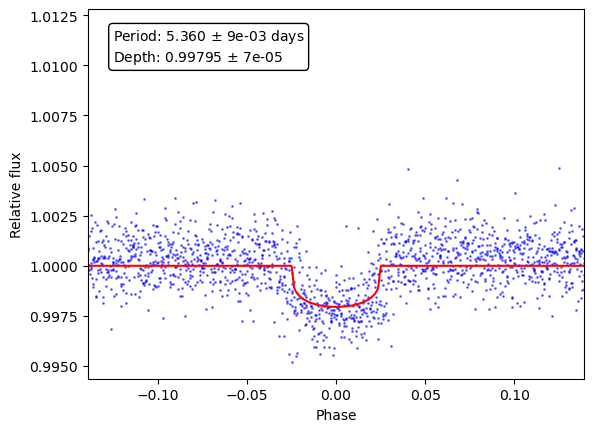
\includegraphics[width=1\textwidth]{figures/tls_results_1}
    \caption{The folded lightcurve at a period of 5.36 days.}
    \label{fig:tls_results_1_folded}
\end{subfigure}%
\hfill
\begin{subfigure}{0.75\textwidth}
    \centering
    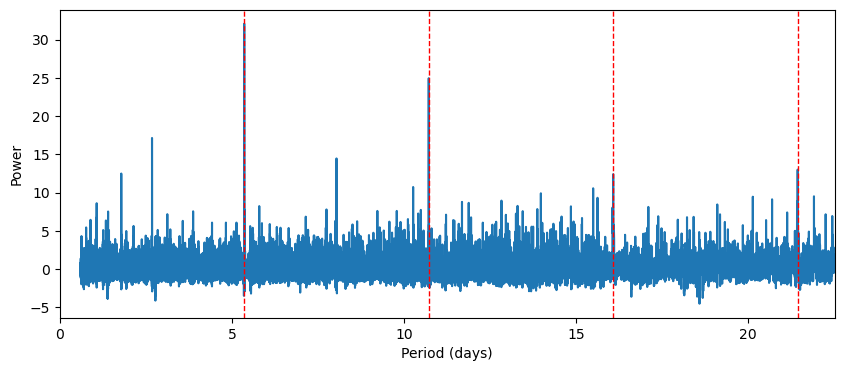
\includegraphics[width=1\textwidth]{./figures/tls_results_1_periodogram}
    \caption{The periodoigram of the TLS algorithm, showing peaks at multiples of the 5.36 day period.}
    \label{fig:tls_results_1_periodogram}
\end{subfigure}
\caption{The folded lightcurve and periodogram of the strongest period identified by the TLS algorithm after removing
the stellar activity.}
\label{fig:tls_results_1}
\end{figure}

Figure~\eqref{fig:tls_results_1} shows the results of the TLS algorithm after removing the stellar activity, with the strongest
period identified at $5.360 \pm 0.009$ days.
The periodogram in Figure~\eqref{fig:tls_results_1_periodogram} supports this result, showing a clear peak at multiples of this period.
Further analysis of the data in a similar way yielded little evidence of any other exoplanets in the data.
Therefore, Table~\eqref{tab:q1_planet_params} summarises the parameters of the identified exoplanet, and the derived
planetary radius and semi-major axis using Kepler's third law (with errors propagated accordingly).

\begin{table}[htb]
    \centering
    \begin{tabular}{ccc}
        \toprule
        \toprule
        Parameter & Units & Value \\
        \midrule
        Orbital Period & $days$ & $5.360 \pm 0.009$ \\
        \addlinespace
        Planetary Radius & $R_{\odot}$ & $0.012 \pm 0.001$  \\
        \addlinespace
        Planet Semi-major Axis $a$ & $AU$ & $0.0381 \pm 0.0007$ \\
        \bottomrule
    \end{tabular}
    \caption{Summary of the parameters of the identified exoplanet, and the derived planetary radius and semi-major axis.}
    \label{tab:q1_planet_params}
\end{table}
